\documentclass[a4paper,11pt]{article}
\usepackage[utf8]{inputenc}

% extra packages
% \usepackage{amsrefs}
% \usepackage[autocite=inline,labelalpha=true]{biblatex}

\usepackage[top=1in, left=1in, right=1in, bottom=1in]{geometry}
\usepackage{amsmath, amssymb}
\usepackage{graphicx}
\usepackage{color}
\usepackage{hyperref}

%\setlength{\parindent}{0pt}

\begin{document}

\begin{center}
\Large \textbf{Statement of Research Interests}

\Large Youngmin Park
\end{center}

% 
% \section{Introduction}
% I am an applied mathematician whose work primarily focuses on the cortex.  In my research thus far, I use dynamical systems theory as a means to understand neural computation. I list a brief summary of my work below, and explain in detail my work at Penn in the next section.
% 
% \begin{itemize}
%  \item \textbf{Park, Y.} and Geffen, M.N. \textit{A Mechanistic Model of the Auditory Cortex with Inhibitory Subtypes} (in preparation). We introduce a groundbreaking model of cortical responses to complex auditory stimuli, which includes inhibitory subtypes implicated in such auditory processing. The model readily generates hypotheses for the role of these inhibitory subtypes across multiple experimental results.
% 
%  \item \textbf{Park, Y.}, Shaw, K.M. Chiel, H.J. Thomas, P.J. \textit{The Infinitesimal Phase Response Curve of Oscillators in Piecewise Smooth Dynamical Systems}. European Journal of Applied Mathematics (2018). We provide a first-principles derivation of the phase response curves (PRCs) of oscillators satisfying non-smooth dynamics. This work is a much-needed extension of the half-century-old theory of PRCs.
%  
%  \item \textbf{Park, Y.}, Ermentrout, G.B. \textit{Weakly Coupled Oscillators in a Slowly Varying World}. (2016). We extend the theory of weakly coupled oscillators to account for a slowly varying parameter, greatly facilitating more realistic and topical studies using dynamic parameters. 
%   
%  \item \textbf{Park, Y.}, Ermentrout, G.B. \textit{Scalar Reduction of a Neural Field Model with Spike Frequency Adaptation}.
%  SIAM Journal on Applied Dynamical Systems (2018). We introduce a novel dimension reduction of so-called ``bump'' solutions of non-local neural field models to centroid coordinates. The dimension reduction allows for a comprehensive analysis of the many bifurcations of the system with greater generality than previously possible.
%  
%  \item \textbf{Park, Y.}, Ermentrout, G.B. \textit{A Multiple Timescales Approach to Bridging Spiking- and Population-level Dynamics}. (2018). We introduce a powerful theory that robustly accounts for large frequency differences between populations. This substantial contribution enables computational works to operate without the classic restraint of small frequency differences.
%  
%  \item \textbf{Park, Y.}, Heitmann, S., Ermentrout, G.B. \textit{The Utility of Phase Models in Studying Neural Synchronization}. Book chapter in Computational Models of Brain and Behavior. Wiley-Blackwell (2017). In this book chapter, we explore how different types of phase response curves and synaptic connections affect the synchronization properties of a network. This chapter is the first to address this relationship directly, and provides a much-needed guideline for future computational studies.
%  
%  \item Shaw, K.M., \textbf{Park, Y.}, Chiel, H.J., Thomas, P.J. \textit{Phase Resetting in an Asymptotically Phaseless System}. SIAM Journal on Applied Dynamical Systems (2012). We derive explicit equations for the phase response curve of a planar, piecewise-linear dynamical system. In contrast to existing beliefs, the work proves that transitions between boundaries can have the greatest effect on the phase response curve.
% \end{itemize}



\section{Modeling the Auditory Cortex}
In my evolution as an applied mathematician working in neuroscience, I found it necessary to work with a leading neuroscience lab in order to understand neuroscience through immersion. I have found the ideal lab for this goal in Maria Geffen's lab at Penn, where I am working on a cortical model of auditory adaptation that takes into account experimental results in optogenetics.

% Recent modeling work has shifted away from the traditional study of simple stimuli, in favor of reproducing neural responses to spectro-temporally complex sounds, such as stimulus-specific adaptation (SSA) \cite{yarden2017stimulus}, forward suppression (FS) \cite{phillips2017cortical}, auditory streaming \cite{rankin2015neuromechanistic}, and pitch change perception \cite{huang2015neuronal}. Models of these phenomena robustly reproduce neural responses for each paradigm, but only include a general inhibitory subpopulation, if any, and do not account for the latest advancement in neuroscience: optogenetics.

\begin{figure}
\centering
 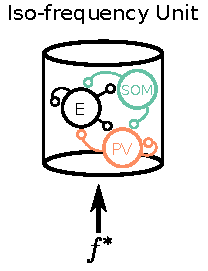
\includegraphics[]{col1.pdf}
 \caption{Iso-frequency unit model. Excitatory (Pyr) form recurrent connections with SOMs and PVs. Connectivity structure and synaptic weights as in Equation \eqref{eq:ssa_weights}. Iso-frequency auditory stimuli directly excite Pyr (E) neurons and PV (orange) interneurons.}\label{ref:col1}
\end{figure}

Optogenetic techniques allow neuroscientists to selectively activate or inhibit specific inhibitory neuron subtypes with unprecedented temporal precision. Such control allows neuroscientists to study the changes in cortical responses as a function of optogenetic suppression, allowing them to uncover the differential role of interneurons, primarily parvalbumin- (PV) positive and somatostatin- (SOM) positive interneurons. Models are now being developed to account for inhibitory subtypes that differentially modulate cortical activity, but they are specific to visual cortex \cite{litwin2016inhibitory}, or are relatively abstract and do not generalize well beyond specific results \cite{seybold2015inhibitory,phillips2016asymmetric,phillips2017cortical}. There exist additional models of inhibitory subtypes modulating functional connectivity \cite{hamilton2013optogenetic} and SSA \cite{natan2015complementary}. Moreover, recent work that shows differential modulation of SOMs and PVs in tuning-curve adaptation does not yet have a model to explain or explore the underlying mechanisms \cite{natan2017cortical}. My job at Penn is to extend and unify these results and models through the use of an augmented Wilson-Cowan model.

% How the neural circuitry in the auditory cortex produces responses to complex auditory stimuli, and the role of particular interneuron subtypes in shaping these responses remains largely unknown. Thus, our modeling goal both advances existing studies and serves as a platform to produce additional questions that will further guide ground-breaking experimental studies.

The model we have developed assumes that basic characteristics of inhibitory modulation are derived from the level of a single neural mass model, which is determined by the system,
\begin{equation}\label{eq:wc}
 \begin{split}
 \frac{d u(t)}{d t} &= -u(t) + f\left( K_{uu} u - K_{up} p - K_{es}s + q I(t) \right),\\
 \tau_p\frac{d p(t)}{d t} &= -p(t) + f\left( K_{pu} u - K_{pp}p - K_{ps}s + q I(t)\right),\\
 \tau_s\frac{d s(t)}{d t} &= -s(t) + f(K_{se}u - K_{sp}p - K_{ss}s),
 \end{split}
\end{equation}
where $u$ represents the normalized firing rate (scaled from 0 to 1) of the excitatory population (Pyr), $p$ and $s$ represent the normalized firing rates PVs and SOMs, respectively. The function $f$ is either a sigmoid or a threshold linear function (such that $f(-\infty) = 0$ and $f(\infty)=1$). The sigmoidal firing rate is defined as
\begin{equation}\label{eq:sigmoid}
 f(x) = \frac{1}{1+\exp(-r x)},
\end{equation}
and the threshold linear function is defined as
\begin{equation}\label{eq:linear}
 f(x) = \left\{\begin{matrix}
         0 & \text{if} \quad x \leq 0\\
         r x & \text{if} \quad 0 < x \leq 1\\
         1 & \text{if} \quad x > 1
        \end{matrix}\right. .
\end{equation}
The parameter $r$ determines the gain of the firing-rate function. Thresholding may be added by writing $f(x-u_{th})$, where $u_{th}$ is a real number.

The input function $I(t)$ consists of blocks of inputs with stimulus interval $\delta$ms (typically 50--100ms depending on the experimental paradigm). When an auditory input arrives, the default temporal profile is taken to have an instantaneous rise with amplitude $q$ and exponential decay with time constant $\tau_q=10$ms. The input $I(t)$ is further modulated by a slow timecourse synaptic depression term $g$ satisfying
\begin{equation}\label{eq:thal}
 dg/dt = (g_0 - g)/\tau_{d_1} - I(t)/\tau_{d_2},
\end{equation}
where the time constants are $\tau_{d_1} = 1500$ms and $\tau_{d_2}=20$ms (chosen close to reported values \cite{natan2015complementary}). The variable $g$ effectively modulates the amplitude of auditory inputs to A1 over long times.

In Figure \ref{fig:wc_space}, each unit shows the connectivity pattern based on existing studies on AC \cite{pfeffer2013inhibition}. The connectivity is equivalently represented by the matrix,
\begin{equation}\label{eq:ssa_weights}
 W = \left(\begin{matrix}
      1.1 & 2 & 1\\
      1   & 2 & 2\\
      6   & 0 & 0
     \end{matrix}\right),
\end{equation}
All synapses in the rate model are constant (as in \cite{mill2011neurocomputational}) except for the depressing feedforward thalamic inputs \cite{lee2008synaptic}.

Standard responses of the augmented Wilson-Cowan are shown in Figure \ref{fig:awc}. The top panel displays the timecourse of all neural populations including Pyr (black), SOM (green), and PV (dashed orange). These responses represent dimensionless population activity, where 0 represents a baseline or below-threshold firing rate, and 1 represents the maximum possible firing rate. The gray line represents the timecourse of the depressing thalamic input, which is also dimensionless in this model. The thalamic input profile is 
shown in the bottom panel (blue).

\begin{figure}[ht!]
\centering
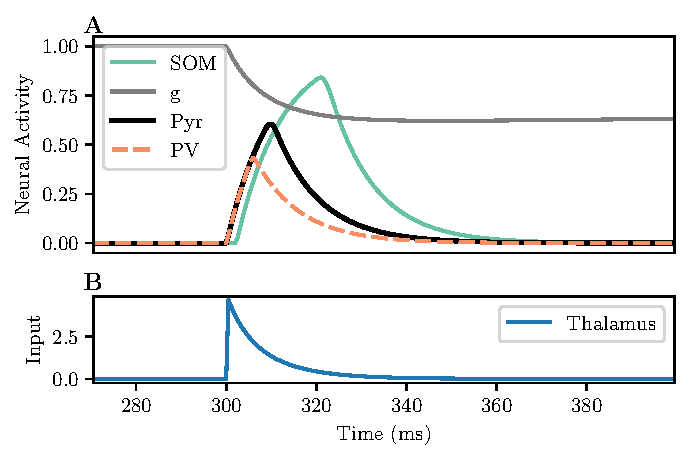
\includegraphics[width=.75\textwidth]{rate_responses.pdf}
 \caption{Input and response profiles of the single-unit model. Gray: The thalamic depression variable $g$. Black: Pyramidal neuron activity. Dashed orange: PV interneuron activity. Green: SOM interneuron activity. Blue, bottom panel: Thalamic inputs. The tone onset occurs at 300ms. While the tone duration lasts for 100ms, fast timescale thalamic adaptation quickly depresses the auditory input. $q=5$.}\label{fig:awc}
\end{figure}

Because both PVs and Pyrs receive direct thalamic inputs, their activation coincide, but PVs peak earlier, in agreement with existing studies \cite{keller2018gap}. Because synapses between excitatory and inhibitory neurons are static, this feature is a result of the connectivity pattern and not due to synaptic effects. The delay in SOM activation is caused by a lack of direct thalamic inputs. SOMs instead receive excitatory input from the Pyr population with a high threshold, making SOM activation dependent on Pyr activity, which occurs on a slower timescale than the thalamic inputs.

An important feature of this model is the early, fast temporal activation of PVs and the late, broad temporal activation of SOMs. While the total inhibition is activresult e both before and well after the peak activation of Pyrs, the differential inhibition of PVs and SOMs result in nontrivial changes to Pyr activity. We will show that this differential change reproduces optogenetic results.

In Figure \ref{fig:wc_space}, we take the single-unit rate model and arrange copies into three units with lateral cortical and thalamic connections (Figure \ref{fig:wc_space}). This arrangement endows our model with a gross tonotopy, which we  use to explore spectrally complex auditory inputs in addition to temporally dynamic sounds. Two examples of the model's output are shown in Figures \ref{fig:ssa} and \ref{fig:fs}.

\begin{figure}[ht!]
\centering
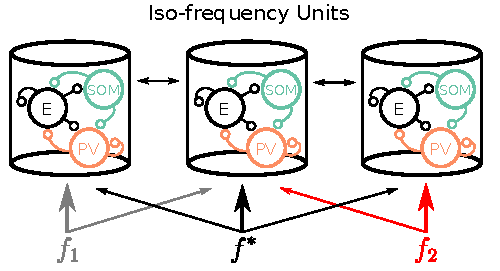
\includegraphics[width=.75\textwidth]{col3.pdf}
\caption{A visual representation of the augmented Wilson-Cowan model with three units.}\label{fig:wc_space}
\end{figure}

In Figure \ref{fig:ssa}, we show how the model performs in an SSA paradigm, where standard tones (red) are presented to the left unit, and deviant tones (gray) are presented to the right unit (panels A and D). With PV inactivation (effected by increasing the firing threshold in the function $f$), there is a constant disinhibition of neural activity from deviant tone to at least four post-deviant tones (panel B). With SOM inactivation, there is an increasing disinhibition from deviant to increase post-deviant tone numbers (panel C). Both panels B and C agree with optogenetic results in SSA \cite{natan2015complementary}.

\begin{figure}[ht!]
 \centering
 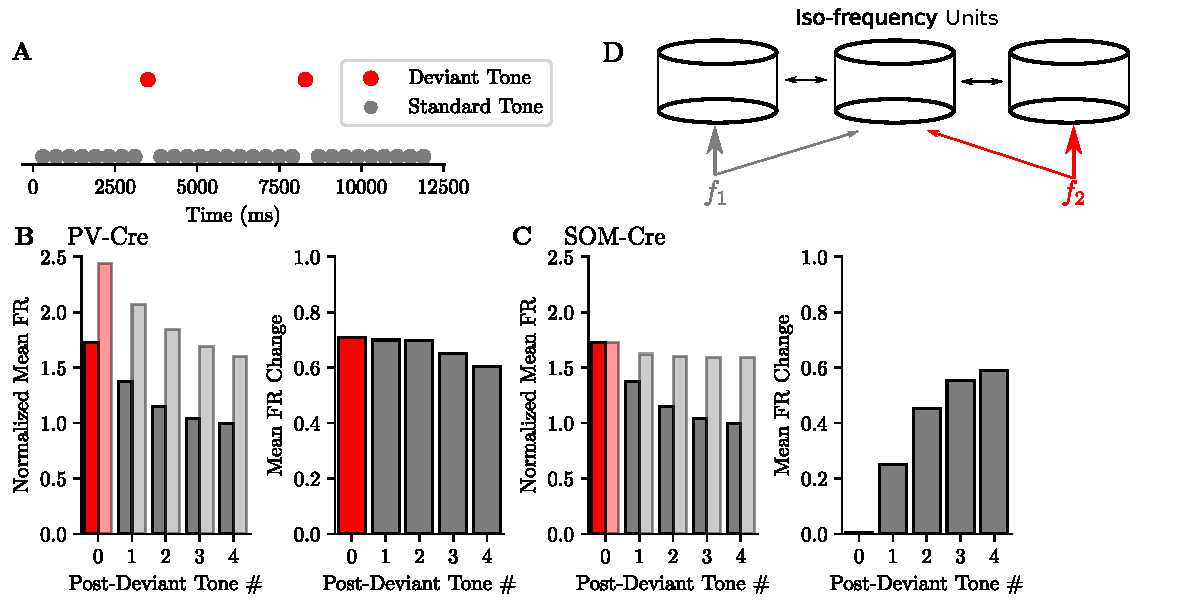
\includegraphics[width=\textwidth]{ssa.pdf}
 \caption{Summary of stimulus-specific adaptation in a two-tone paradigm. A: The timing of standard and deviant tones used in this model. Standard tones (gray) appear with 95\% probability, while deviant tones (red) appear with 5\% probability. B: PV inactivation results in a near-uniform increase in firing rates (FR) through all post-deviant tones. C: SOM inactivation reveals a gradually increasing inhibitory effect. Both panels B and C qualitatively reproduce experimental results \cite{natan2015complementary}.}\label{fig:ssa}
\end{figure}

The same model with the same parameter set reproduces optogenetic results in forward suppression (Figure \ref{fig:fs}). In the left panel, PV inactivation results in an enhanced forward suppression, while the right panel shows SOM inactivation results in a reduced forward suppression. Both results agree with optogenetic experiments in forward suppression \cite{phillips2017cortical}.

\begin{figure}[ht!]
 \centering
 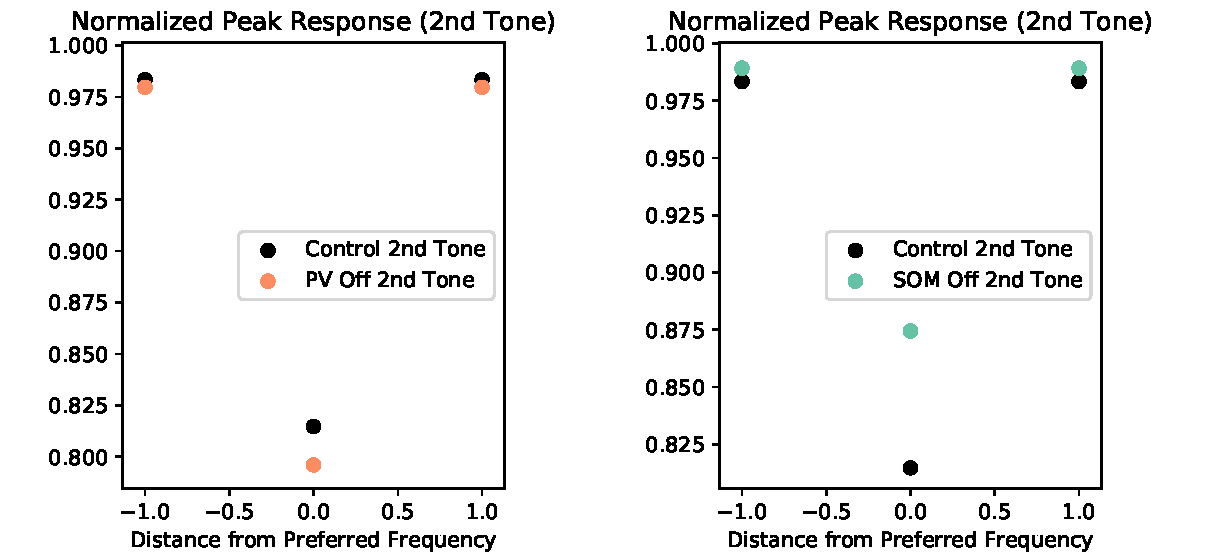
\includegraphics[width=\textwidth]{fs.pdf}
 \caption{Summary of forward suppression. A: Disinhibition of PV (orange) results in greater probe alone (PA) responses compared to the control (black). B: Normalizing by the PA tone shows that PV inhibition enhances forward suppression, in agreement with experiments. C: Disinhibition of SOM (teal) results in greater PA responses compared to the control (black). D: Normalizing by the PA tone shows that SOM inhibition results in reduced forward suppression and enhanced sideband facilitation, in agreement with experiments.}\label{fig:fs}
\end{figure}

The model has also been used to show an increase in functional connectivity as a function of PV activation (data not shown). As PVs increase in activity, the excitatory population activity peaks closer to the onset of the thalamic input (i.e. the auditory stimulus), resulting in an enhanced correlation between the sound and cortical activity. This phenomenon agrees with existing experimental results and demonstrates a plausible mechanism for changes to the functional connectivity in the cortex \cite{hamilton2013optogenetic}.

\subsection{Future Work}
  
The next step is to include results in tuning-curve adaptation (\cite{natan2017cortical}). We also have a single-unit spiking model, which we are currently extending to three units, in order to introduce a gross tonotopy. Results are promising.

\section{Conclusion}

This experience has given me a healthy respect for data and data analysis. I am humbled by the scientific feats my lab mates perform every week. In less than a year, I have come to understand the value of early, in-depth communication when determining collaborative projects, and the need for understanding when communicating with people of disparate scientific fields. Despite these hurdles, I am inspired, and this experience will be extremely valuable to me as an applied mathematician who will continue fostering close relationships with experimentalists.


\bibliographystyle{plain}
\bibliography{../../GeffenLab/Youngmin/audio,../../GeffenLab/Youngmin/computation,../../GeffenLab/Youngmin/cortex,../../GeffenLab/Youngmin/bio,../../GeffenLab/Youngmin/machines,../../GeffenLab/Youngmin/math}


\end{document}
